\documentclass{standalone}
\usepackage[T1]{fontenc}
\usepackage[utf8]{inputenc}
\usepackage{pgf,tikz}
\usepackage{setspace}
\usepackage{pgfplots}
\usepgfplotslibrary{polar}
\pgfplotsset{compat=1.13}


\begin{document}

\def\samplePeriod{0.3}


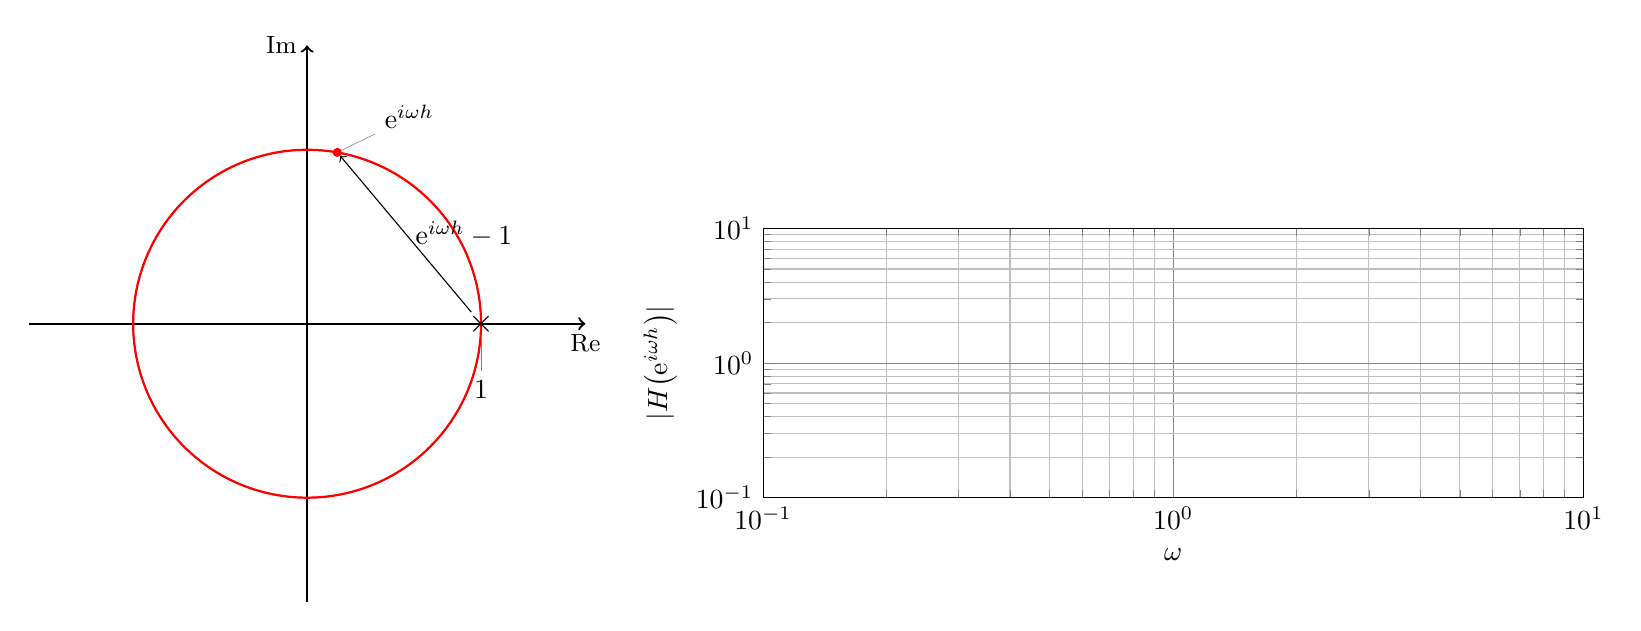
\begin{tikzpicture}
  \begin{polaraxis}[
    xshift=0cm,
    width=6cm,
    height=6cm,
    clip=false,
    xtick=\empty,
    ytick=\empty,
    ymin=0, ymax=1,
    y tick label style={anchor=north east},
    ]

    \draw[->, thick] (axis cs: 270, 1.6) -- (axis cs: 90, 1.6) node [left] {\small $\mathrm{Im}$};
    \draw[->, thick] (axis cs: 180, 1.6) -- (axis cs: 0, 1.6) node [below] {\small $\mathrm{Re}$};

    \addplot+[thick, red, no marks, domain=0:360, samples=400] (x, 1);
    
    \node[circle, draw, inner sep=1pt, fill, red, pin=20:{$\mathrm{e}^{i\omega h}$}] at (axis cs: 80, 1)  (freq) {};

    \node[inner sep=0pt, pin=-90:{1}] at (axis cs: 0,1) (pole) {\large $\times$}; 
    \draw[->]  (pole) -- node [right] {$\mathrm{e}^{i\omega h} - 1$} (freq);

\end{polaraxis}

  
  \begin{loglogaxis} [
      ylabel=$|H\big(\mathrm{e}^{i\omega h}\big)|$,
      xlabel=$\omega$,
      xshift = 8cm, 
      width=12cm,
      height=5cm,
      grid=both,
      every major grid/.style={red, opacity=0.5},
      %ytick={0.5, 2},
      %yticklabels={$\frac{J\omega_0}{k_d2}$, $\frac{2J\omega_0}{k_d}$},
      %xticklabel=\empty,
      ymin=0.1, ymax=10,
      xmin=0.1, xmax=10,
      %legend entries={Bessel filter, Delay of one},
      %legend pos={south west},
  ]
  \end{loglogaxis}

\end{tikzpicture}

\end{document}
